\documentclass{article}
\usepackage{makeidx}
\usepackage{hyperref}
\usepackage{amsmath}
\usepackage{amssymb}
\usepackage{xcolor}
\usepackage{graphicx}

\title{Deep Learning Notes}
\author{Haotian Chen}
\date{}

\makeatletter
\renewcommand\paragraph{\@startsection{paragraph}{4}{\z@}%
                                     {-3.25ex\@plus -1ex \@minus -.2ex}%
                                     {1.5ex \@plus .2ex}%
                                     {\normalfont\normalsize\bfseries}}
\makeatletter

\hypersetup{
    colorlinks=true,
    linkcolor=blue,
    urlcolor=cyan,
}

\setcounter{tocdepth}{4}
\setcounter{secnumdepth}{4}

\makeindex



\begin{document}

\maketitle

\clearpage

\tableofcontents{}

\clearpage

\section{Neural Networks and Deep Learning}

\subsection{Activation Function}

\noindent \textbf{binary step:}

\begin{center}
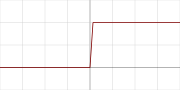
\includegraphics[scale=0.8]{./images/binary_step.png}
\end{center}

\[f(x) = \begin{cases}0&{\text{if }}x<0\\1&{\text{if }}x\geq 0\end{cases}, f(x) \in \{0, 1\}\]
\[f'(x) = \begin{cases}0&{\text{if }}x\neq 0\\{\text{undefined}}&{\text{if }}x=0\end{cases}\]

\noindent \textbf{sigmoid function:} (mainly used in output layer)

\begin{center}
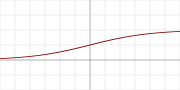
\includegraphics[scale=0.8]{./images/sigmoid.png}
\end{center}

\[f(x) = \sigma (x)={\frac {e^{x}}{e^{x}+1}}={\frac {1}{1+e^{-x}}}, f(x) \in (0, 1)\]
\[f'(x) = f(x)(1-f(x))\]

\noindent \textbf{rectified linear unit:}  (relu, mainly used in hidden layer)

\begin{center}
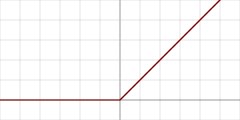
\includegraphics[scale=0.6]{./images/relu.png}
\end{center}

\[f(x) = max\{0, x\} = \begin{cases}0&{\text{if }}x<0\\1&{\text{if }}x\geq 0\end{cases}, f(x) \in [0, +\infty)\]
\[f'(x) = \begin{cases}0&{\text{if }}x<0\\1&{\text{if }}x>0\\{\text{undefined}}&{\text{if }}x=0\end{cases}\]

\noindent \textbf{Leaky rectified linear unit:}  (leaky relu, mainly used in hidden layer)

\begin{center}
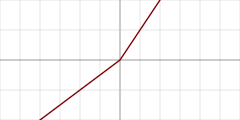
\includegraphics[scale=0.6]{./images/leaky_relu.png}
\end{center}

\[f(x) = \begin{cases}0.01x&{\text{if }}x<0\\x&{\text{if }}x\geq 0\end{cases}, f(x) \in (- \infty, + \infty)\]
\[f'(x) = \begin{cases}0.01&{\text{if }}x<0\\1&{\text{if }}x\geq 0\end{cases}\]

\noindent \textbf{hyperbolic tangent:} (tanh, mainly used in hidden layer)

\begin{center}
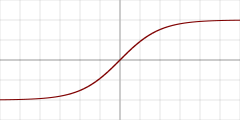
\includegraphics[scale=0.6]{./images/tanh.png}
\end{center}

\[f(x) = \tanh(x) = \frac {e^{x}-e^{-x}}{e^{x}+e^{-x}}, f(x) \in (-1, 1)\]
\[f'(x) = 1-f(x)^{2}\]

\noindent It turns out that the tanh activation usually works better than sigmoid activation function for hidden units because the mean of its output is closer to zero, and so it centers the data better for the next layer. Sigmoid or Tanh function disadvantage is that if the input is too small or too high, the slope will be near zero which will cause us the vanishing gradient problem.

\bigskip

\noindent Linear activation function will output linear activations. No matter how many hidden layers you add, the activation will be always linear like logistic regression (So its useless in a lot of complex problems). You might use linear activation function in the output layer if the output is real numbers (regression problem).

\subsection{Computation Graphs of Derivatives:}

\begin{center}
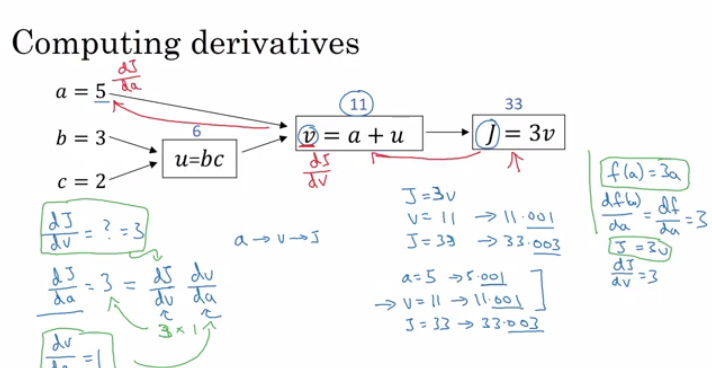
\includegraphics[scale=0.6]{./images/computation_graph.png}
\end{center}

\noindent apply chain rule:

\[\frac{\partial J}{\partial a} = \frac{\partial J}{\partial v} \frac{\partial v}{\partial a} = 3 \times 1 = 3\]

\[\frac{\partial J}{\partial b} = \frac{\partial J}{\partial v} \frac{\partial v}{\partial u} \frac{\partial u}{\partial b} = 3 \times 1 \times 2 = 6\]

\[\frac{\partial J}{\partial c} = \frac{\partial J}{\partial v} \frac{\partial v}{\partial u} \frac{\partial u}{\partial c} = 3 \times 1 \times 3 = 9\]


\subsection{Binary Classification}

Use logistic regression to build a binary classifier.

\begin{center}
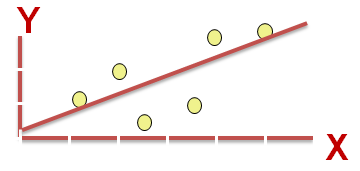
\includegraphics[scale=0.4]{./images/binary_classification.png}
\end{center}

\noindent \textbf{training data:}
\[x \in \mathbb{R}^{n_x}, y \in \{0, 1\}\]
\[\text{\(m\) training examples: } (x^{(i)}, y^{(i)})\:for\:i = 1, \dots, m\]

\[
x^{(i)} = 
\begin{bmatrix}
x^{(i)}_1\\
x^{(i)}_2\\
\vdots\\
x^{(i)}_n
\end{bmatrix}
,
y^{(i)} = y^{(i)}_1
\]

\[X =
\begin{bmatrix}
x^{(1)} & x^{(2)} & \dots & x^{(m)}
\end{bmatrix}
,
Y =
\begin{bmatrix}
y^{(1)} & y^{(2)} & \dots & y^{(m)}
\end{bmatrix}
\]

\[X \in \mathbb{R}^{n_x \times m}, Y \in \mathbb{R}^{1 \times m}\]

\subsection{Logistic Regression}

\noindent Logistic regression is a statistical model that uses a logistic function to model a binary dependent variable.

\bigskip

\noindent Given \(x\), want \(\hat{y} = P(y = 1 | x)\), where \(0 \leq \hat{y} \leq 1\), \(x \in \mathbb{R}^{n_x}\), \(w \in \mathbb{R}^{n_x}\), \(b \in \mathbb{R}\)

\[z = w^Tx + b\]
\[\hat{y} = \sigma(z) = \frac {1}{1+e^{-z}}\]

\[P(y|x) = \begin{cases}\hat{y}&{\text{if }}y = 1\\1 -\hat{y}&{\text{if }}y = 0\end{cases} = \hat{y}^y (1 - \hat{y})^{(1 - y)}\]

\noindent We want to maximize \(P(y|x)\). To make it simpler, because \(log\) function is a strictly increasing function, we can maximize \(log(P(y|x))\) instead.

\[log(P(y|x)) = log(\hat{y}^y (1 - \hat{y})^{(1 - y)}) = ylog(\hat{y}) + (1 - y)log(1 - \hat{y})\]

\noindent Or in reverse, we can minimize \(-log(P(y|x))\), which is called \textbf{loss function}.

\noindent \textbf{loss function: (convex)}

\[L(\hat{y}, y) = -(ylog(\hat{y}) + (1 - y)log(1 - \hat{y}))\]

\noindent \textbf{cost function: (convex)}

\[J(w, b) = \frac{1}{m} \sum^m_{i = 1} L(\hat{y}^{(i)}, y^{(i)}) = - \frac{1}{m} \sum^m_{i = 1} [y^{(i)}log(\hat{y}^{(i)}) + (1 - y^{(i)})log(1 - \hat{y}^{(i)})]\]

\noindent \textbf{gradient descent:} with learning rate \(\alpha\), find best \(w\), \(b\) to minimize \(J(w, b)\)

\noindent repeat until convergence \{
\[w_j =: w_j - \alpha \frac{\partial}{\partial w_j} J(w, b) = w_j - \alpha \frac{1}{m} \sum^m_{i = 1} (\hat{y}^{(i)} - y^{(i)}) x^{(i)}_j\]
\[b =: b - \alpha \frac{\partial}{\partial b} J(w, b) = b - \alpha \frac{1}{m} \sum^m_{i = 1} (\hat{y}^{(i)} - y^{(i)})\]
\centerline{simultaneously update \(w_j\) and \(b\), \(j \in [1, n]\)}
\}

\bigskip

\noindent \textbf{vectorized implementation}:

\noindent repeat until convergence \{
\[w =: w - \alpha \frac{1}{m} X (\sigma(w^TX + b) - Y)^T\]
\[b =: b - \alpha \frac{1}{m} sum\{\sigma(w^TX + b) - Y\}\]
\}

\subsection{Neural Network}

\noindent \textbf{Basic Structure:}

\begin{center}
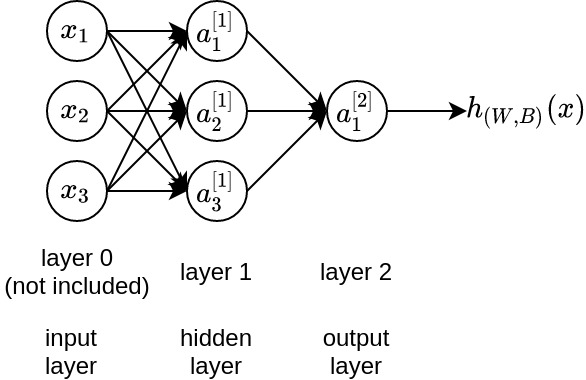
\includegraphics[scale=0.4]{./images/neural_network.jpg}
\end{center}
\[a_i^{[j]} = \text{"activation" of unit i in layer j}\]
\[W^{[j]} = \text{matrix of weights (edges) from layer j to j + 1}\]
\[B^{[j]} = \text{vector of biases (nodes) from layer j to j + 1}\]

\[a_1^{[1]} = \sigma(W_{11}^{[0]} x_1 + W_{12}^{[0]} x_2 + W_{13}^{[0]} x_3 + B_{1}^{[0]})\]
\[a_2^{[1]} = \sigma(W_{21}^{[0]} x_1 + W_{22}^{[0]} x_2 + W_{23}^{[0]} x_3 + B_{2}^{[0]})\]
\[a_3^{[1]} = \sigma(W_{31}^{[0]} x_1 + W_{32}^{[0]} x_2 + W_{33}^{[0]} x_3 + B_{3}^{[0]})\]
\[h_{(W, B)}(x) = a_1^{[2]} = \sigma(W_{11}^{[1]} a_1^{[1]} + W_{12}^{[1]} a_2^{[1]} + W_{13}^{[1]} a_3^{[1]} + B_{1}^{[1]})\]

\bigskip

\noindent If network has \(s_j\) units in layer \(j\), \(s_{j + 1}\) units in layer \(j + 1\), then \(W^{[j]}\) will be of dimension \(s_{j + 1} \times s_j\), \(B^{[j]}\) will be of dimension \(s_{j + 1} \times 1\).

\bigskip

\noindent \textbf{Generalized Model (one vs all):}

\begin{center}
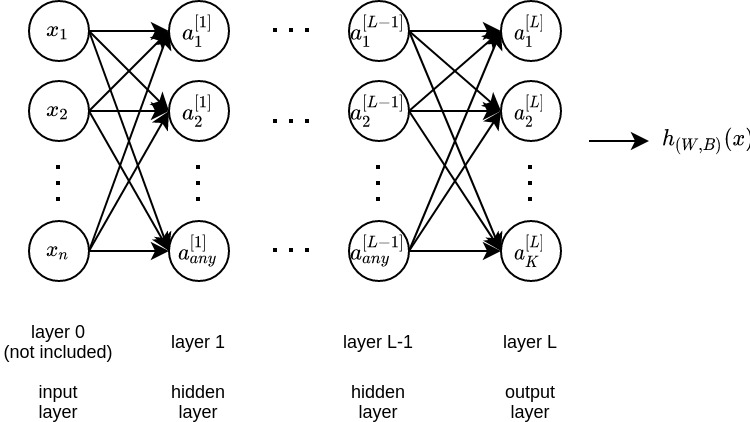
\includegraphics[scale=0.4]{./images/neural_network_generalized.jpg}
\end{center}

\noindent For a neural network that has:

\[L = \text{total number of layers in the network}\]
\[s_l = \text{number of units in layer } l\]
\[K = \text{number of output units/classes}\]

\noindent assume \(a^{[0]} = x, a^{[L]} = h_{(W, B)}(x)\), let:

\[z^{[l]} = W^{[l - 1]} a^{[l - 1]} + B^{[l - 1]}\]
\[a^{[l]} = \sigma(z^{[l]})\]
\[h_{(W, B)}(x) = a^{[L]} = \sigma(z^{[L]})\]

\bigskip

\noindent \textbf{regularized cost function:}
\[J(W, B) = - \frac{1}{m} \sum_{i = 1}^{m} \sum_{k = 1}^{K} [y^{(i)}_k log(h_{(W, B)} (x^{(i)})_k) + (1 - y^{(i)}_k) log(1 - h_{(W, B)}(x^{(i)})_k)] + \frac{\lambda}{2m} \sum_{l = 0}^{L - 1} \sum_{i = 1}^{s_l} \sum_{j = 1}^{s_{l + 1}} (W_{j, i}^{[l]})^{2}\]

\noindent To reduce over-fitting, we can reduce(penalize) the weight of the features in our function carry by increasing their cost. The \(\lambda\) is the regularization parameter. It determines how much the costs of our theta parameters are inflated.

\subsection{Backpropagation Preliminary}
\noindent \textbf{matrix calculus:} see \href{https://en.wikipedia.org/wiki/Matrix_calculus}{Wikipedia}

\noindent \textbf{chaine rule:}

\noindent Suppose the variable \(J\) depends on the variables \(w_1, \dots, w_p\) via the intermediate variable \(z_1, \dots, z_k\).

\[z_j = z_j(w_1, \dots, w_p), \forall j \in \{1, \dots, k\} \]
\[J = J(z_1, \dots, z_k)\]

\noindent Expand \(J\), we can find:

\[\frac{\partial J}{\partial w_i} = \sum_{j = 1}^{k} \frac{\partial J}{\partial z_j} \frac{\partial z_j}{\partial w_i}, \forall i \in \{1, \dots, p\}\]

\noindent \textbf{chain rule derivation for matrix:}

\noindent Suppose \(J\) is a real-valued output variable, \(z \in \mathbb{R}^m\) is the intermediate variable and \(W \in \mathbb{R}^{m \times d}\), \(B \in \mathbb{R}^{m}\), \(a \in \mathbb{R}^d\) are the input variables. Suppose they satisfy:

\[z = W a + B\]
\[J = J(z)\]

\noindent Then we can get:

\[
\frac{\partial J}{\partial a} = 
\begin{bmatrix}
\frac{\partial J}{\partial a_1}\\
\vdots\\
\frac{\partial J}{\partial a_d}
\end{bmatrix}
= 
\begin{bmatrix}
\sum_{j = 1}^m \frac{\partial J}{\partial z_j} \frac{z_j}{a_1}\\
\vdots\\
\sum_{j = 1}^m \frac{\partial J}{\partial z_j} \frac{z_j}{a_d}
\end{bmatrix}
=
\begin{bmatrix}
\frac{\partial z_1}{\partial a_1} & \dots & \frac{\partial z_m}{\partial a_1}\\
\vdots & \ddots & \vdots\\
\frac{\partial z_1}{\partial a_d} & \dots & \frac{\partial z_m}{\partial a_d}
\end{bmatrix}
\begin{bmatrix}
\frac{\partial J}{\partial z_1}\\
\vdots\\
\frac{\partial J}{\partial z_m}
\end{bmatrix}
= \frac{\partial z}{\partial a} \frac{\partial J}{\partial z}
= W^T \frac{\partial J}{\partial z}
\]

\[
\frac{\partial J}{\partial W_{ij}} = \sum_{k = 1}^m \frac{\partial J}{\partial z_k} \frac{\partial z_k}{\partial W_{ij}} = \frac{\partial J}{\partial z_i} \frac{\partial z_i}{\partial W_{ij}} = \frac{\partial J}{\partial z_i} a_j
\]

\[
\frac{\partial J}{\partial B_{i}} = \sum_{k = 1}^m \frac{\partial J}{\partial z_k} \frac{\partial z_k}{\partial B_{i}} = \frac{\partial J}{\partial z_i} \frac{\partial z_i}{\partial B_{i}} = \frac{\partial J}{\partial z_i}
\]

\[
\frac{\partial J}{\partial W} = 
\begin{bmatrix}
\frac{\partial J}{\partial z_1}\\
\vdots\\
\frac{\partial J}{\partial z_m}
\end{bmatrix}
\begin{bmatrix}
a_1 & \dots & a_d
\end{bmatrix}
= \frac{\partial J}{\partial z} a^T
\]

\[
\frac{\partial J}{\partial B} = 
\begin{bmatrix}
\frac{\partial J}{\partial z_1}\\
\vdots\\
\frac{\partial J}{\partial z_m}
\end{bmatrix}
= \frac{\partial J}{\partial z}
\]

\noindent \textbf{element-wise chain rule:}

\noindent Assume \(z, a \in \mathbb{R}^d\):

\[a = \sigma(z) \text{, where \(\sigma\) is an element-wise activation}\]
\[J = J(a)\]

\noindent Then we have:

\[\frac{\partial J}{\partial z} = \frac{\partial J}{\partial a} \odot \sigma'(z)\]

\noindent Where \(\sigma'\) is the element-wise derivative of the activation function \(\sigma\).

\subsection{Backpropagation}

\noindent To train the model, we need to update \(W\) and \(B\) for each epoch: (gradient decent)

\[W := W - \alpha  \frac{\partial}{\partial W} J(W, B)\]
\[B := B - \alpha  \frac{\partial}{\partial B} J(W, B)\]

\noindent We can see \(\frac{\partial}{\partial W} J(W, B)\) and \(\frac{\partial}{\partial B} J(W, B)\) are hard to get directly. There is an easier way to calculate it. For each training example \((x^{(q)}, y^{(q)}), q \in \{1, \dots, m\}\), define \textbf{loss function}:

\[J = -\sum_{k = 1}^{K} [y^{(q)}_k log(h_{(W, B)} (x^{(q)})_k) + (1 - y^{(q)}_k) log(1 - h_{(W, B)}(x^{(q)})_k)] \]

\noindent Apply chain rule we have:

\[\frac{\partial J}{\partial W^{[l]}} = \frac{\partial J}{\partial z^{[l + 1]}} (a^{[l]})^T\]
\[\frac{\partial J}{\partial B^{[l]}} = \frac{\partial J}{\partial z^{[l + 1]}}\]
\[\frac{\partial J}{\partial a^{[l]}} = (W^{[l]})^T \frac{\partial J}{\partial z^{[l + 1]}}\]
\begin{equation*}
\begin{split}
\frac{\partial J}{\partial z^{[l]}}
& = \frac{\partial J}{\partial a^{[l]}} \odot g'(z^{[l]}) \\
& = (W^{[l]})^T \frac{\partial J}{\partial z^{[l + 1]}} \odot g'(z^{[l]}) \\
& = (W^{[l]})^T \frac{\partial J}{\partial z^{[l + 1]}} \odot (a^{[l]} \odot (1 - a^{[l]}))
\end{split}
\end{equation*}

\noindent For \(p \in \{1, ..., K\}\):
\begin{equation*}
\begin{split}
\frac{\partial J}{\partial z_p^{[L]}} 
& = \frac{\partial}{\partial z_p^{[L]}} \sum_{k = 1}^{K} -[y^{(q)}_k log(h_{(W, B)} (x^{(q)})_k) + (1 - y^{(q)}_k) log(1 - h_{(W, B)}(x^{(q)})_k)] \\
& = \frac{\partial}{\partial z_p^{[L]}} \{-[y^{(q)}_p log(\frac{1}{1 + e^{-z_p^{[L]}}}) + (1 - y^{(q)}_p) log(1 - \frac{1}{1 + e^{-z_p^{[L]}}})]\} \\
& = - [y^{(q)}_p (1 + e^{-z_p^{[L]}}) \frac{0 - (-e^{-z_p^{[L]}})}{(1 + e^{-z_p^{[L]}})^2} + (1 - y^{(q)}_p) \frac{1 + e^{-z_p^{[L]}}}{e^{-z_p^{[L]}}} \frac{(-e^{-z_p^{[L]}})(1 + e^{-z_p^{[L]}}) - e^{-z_p^{[L]}}(-e^{-z_p^{[L]}})}{(1 + e^{-z_p^{[L]}})^2}] \\
& = - [y_p^{(q)} \frac{e^{-z_p^{[L]}}}{1 + e^{-z_p^{[L]}}} + (1 - y_p^{(q)}) \frac{-1}{1 + e^{-z_p^{[L]}}}] \\
& = - \frac{y_p^{(q)}e^{-z_p^{[L]}} + y_p^{(q)} - 1}{1 + e^{-z_p^{[L]}}} \\
& = \frac{1}{1 + e^{-z_p^{[L]}}} - y_p^{(q)} \\ 
& = a_p^{[L]} - y_p^{(q)}
\end{split}
\end{equation*}

\noindent Then we get:

\[\frac{\partial J}{\partial z^{[L]}} = 
\begin{bmatrix}
\frac{\partial J}{\partial z_1^{[L]}} \\
\vdots \\
\frac{\partial J}{\partial z_K^{[L]}}
\end{bmatrix}
= a^{[L]} - y^{(q)}
\]

\noindent For convenience, define \textbf{error term}: 
\[\delta^{[l]} = \frac{\partial J}{\partial z^{[l]}}\]

\noindent Then we get:

\[\frac{\partial J}{\partial W^{[l]}} = \delta^{[l + 1]} (a^{[l]})^T\]
\[\frac{\partial J}{\partial B^{[l]}} = \delta^{[l + 1]}\]
\[\delta^{[l]} = (W^{[l]})^T \delta^{[l + 1]} \odot (a^{[l]} \odot (1 - a^{[l]}))\]
\[\delta^{[L]} = a^{[L]} - y^{(q)}\]

\noindent \textbf{backpropagation algorithm:} (compute \(\frac{\partial}{\partial W} J(W, B)\), \(\frac{\partial}{\partial B} J(W, B)\))

\noindent training set: \((x^{(q)}, y^{(q)}), q \in \{1, \dots, m\}\)

\noindent set \(\Delta(W)_{ij}^{[l]} = 0, \Delta(B)_{i}^{[l]} = 0, l \in \{0, \dots, L - 1\}\)

\noindent for \(q \in \{1, \dots, m\}\):

\noindent \hspace{.5cm} forward propagation: compute \(a^{[l]}\) for \(l \in \{1, \dots, L\}\)

\noindent \hspace{.5cm} compute \(\delta^{[L]} = a^{[L]} - y^{(q)}\)

\noindent \hspace{.5cm} for \(l \in \{L - 1, \dots, 1\}\):

\noindent \hspace{1cm} compute \(\delta^{[l]} = (W^{[l]})^T \delta^{[l + 1]} \odot (a^{[l]} \odot (1 - a^{[l]}))\)

\noindent \hspace{.5cm} for \(l \in \{0, \dots, L - 1\}\):

\noindent \hspace{1cm} compute \(\Delta(W)^{[l]} := \Delta(W)^{(l)} + \frac{\partial J}{\partial W^{[l]}} = \Delta(W)^{[l]} + \delta^{[l + 1]}(a^{[l]})^T\)

\noindent \hspace{1cm} compute \(\Delta(B)^{[l]} := \Delta(B)^{(l)} + \frac{\partial J}{\partial B^{[l]}} = \Delta(B)^{[l]} + \delta^{[l + 1]}\)

\noindent compute \(\frac{\partial}{\partial W_{ij}^{[l]}} J(W, B) = D(W)_{ij}^{[l]} = \frac{1}{m} \Delta(W)_{ij}^{[l]} + \frac{\lambda}{m} W_{ij}^{[l]}\)

\noindent compute \(\frac{\partial}{\partial B_{i}^{[l]}} J(W, B) = D(B)_{i}^{[l]} = \frac{1}{m} \Delta(B)_{i}^{[l]} + \frac{\lambda}{m} B_{i}^{[l]}\)

\subsection{Random Initialization (symmetry breaking)}

\noindent Initializing bias matrices \(B\) with zero is OK. Initializing all the weight matrices \(W\) with zero does not work with neural networks, because all hidden units will be completely identical (symmetric) - compute exactly the same function. When we backpropagate, all nodes will update to the same value repeatedly. Instead we can randomly initialize our weights for our \(W\) matrices using the following method: (here \(\epsilon\) is a value selected for random initialization)

\[\text{initialize each } W_{ij}^{[l]} \text{ to a random value in } [-\epsilon, +\epsilon]\]

\noindent One effective strategy for choosing \(\epsilon\) is to base it on the number of units in the network: (Xavier normalized initialization)

\[\epsilon^{[l]} = \frac{\sqrt{6}}{\sqrt{s^{[l]} + s^{[l + 1]}}}\]

\printindex

\end{document}